\documentclass{article}
\usepackage{amsmath}
\usepackage[utf8]{inputenc}
\usepackage{float}
\usepackage{epsfig,graphicx}
\usepackage{xcolor,import}
\usepackage[german]{babel}
\usepackage{textcomp}
\usepackage{mathtools}

\begin{document}
\thispagestyle{empty}
			\begin{center}
			\Large{Fakultät für Physik}\\
			\end{center}
\begin{verbatim}


\end{verbatim}
							%Eintrag des Wintersemesters
			\begin{center}
			\textbf{\LARGE WINTERSEMESTER 2014/15}
			\end{center}
\begin{verbatim}


\end{verbatim}
			\begin{center}
			\textbf{\LARGE{Physikalisches Praktikum 1}}
			\end{center}
\begin{verbatim}




\end{verbatim}

			\begin{center}
			\textbf{\LARGE{PROTOKOLL}}
			\end{center}
			
\begin{verbatim}





\end{verbatim}

			\begin{flushleft}
			\textbf{\Large{Experiment Nr. 10:}} \Large{Wechselstrom I:
Temperaturabhängigkeit des elektrischen Widerstandes,
Transformator}\\
							%Experiment Nr. und Titel statt den Punkten eintragen
			\LARGE{}	
			\end{flushleft}

\begin{verbatim}

\end{verbatim}	
							%Eintragen des Abgabedatums, oder des Erstelldatums des Protokolls
			\begin{flushleft}
			\textbf{\Large{Datum:}} \Large{19.12.2014}
			\end{flushleft}
			
\begin{verbatim}
\end{verbatim}
							%Namen der Protokollschreiber
		\begin{flushleft}
			\textbf{\Large{Namen:}} \Large{Veronika Bachleitner, Erik Grafendorfer}
			\end{flushleft}

\begin{verbatim}


\end{verbatim}
							%Kurstag und Gruppennummer, zb. Fr/5
			\begin{flushleft}
			\textbf{\Large{Kurstag/Gruppe:}} \Large{Fr/1}
			\end{flushleft}

\begin{verbatim}






\end{verbatim}
							%Name des Betreuers, das Praktikum betreute.
			\begin{flushleft}
			\LARGE{\textbf{Betreuer:}}	\Large{KLEPP}	
			\end{flushleft}
\newpage	

\section{Temperaturabhängigkeit des elektrischen Widerstandes}

\subsection{Aufgabenstellung}
Wir bestimmen Eigenschaften verschiedener eines Metalls, eines Halbleiters und eines elektrolytischen Leiters durch Messen ihrer Stromleitungseigenschaften unter verschiedenen Temperaturen.
\subsection{Grundlagen}
\subsubsection*{Metallischer Leiter}
Der temperaturabhängige Widerstand R(T) eines Metallischen Leiters verläuft bei mittleren Temperaturen näherungsweise linear:
\begin{equation}
\label{MetallWiderstand}
R(T) = R_{T0} (1+ \alpha (T-T_0))
\end{equation}
Wobei $ R_{T0}$ der Ausgangs- bzw. Referenzwiderstand ist,
T die Temperatur, und 
$T_0$ die Ausgangs- bzw. Referenztemperatur. 
$\alpha$ ist der Temperaturkoeffizient.\\

\subsubsection*{Halbleiter}
Der Widerstand von Halbleitern bei höheren Temperaturen kann mit einer Exponentialfunktion beschrieben werden.

\begin{equation}
\label{HalbleiterWiderstand}
R(T)=R_{T0}e^{-b(\frac{1}{T_0}-\frac{1}{T})}
\end{equation}

\subsubsection*{Elektrolytischer Leiter}

Die Viskosität $\eta$ einer Flüßigkeit sinkt mit steigender Temperatur - dabei nimmt die Beweglichkeit $\mu$ der Ladungsträger zu, also steigt die Leitfähigkeit $\sigma$.

\begin{equation}
\label{Viskositaet}
\eta = \eta_0 \cdot e^{\frac{E_A}{k_B \cdot T}}
\end{equation}
$E_A$ bezeichnet die Aktivierungsenergie.
\begin{equation}
\label{LeitfaehigkeitElektrolyt}
\sigma  \propto \mu \propto \frac{1}{\eta} \propto e^{-\frac{E_A}{k_B \cdot T}}
\end{equation}

Die Leitfähigkeit $\sigma$ ist indirekt proportional zum Widerstand, also sinkt dieser bei steigender Temperatur.

\begin{equation}
\label{WiderstandElektrolyt}
R(T) \propto \frac{1}{\sigma} \propto e^{\frac{E_A}{k_B \cdot T}}
\end{equation}

\subsection{Versuchsaufbau und Methoden}
\subsubsection*{Metall}
Beim metallischen Leiter formen wir (\ref{MetallWiderstand}) um zu 
\begin{equation}
\label{alpha-metall}
\frac{R(T)}{R_0}-1=\alpha(T-T_0)
\end{equation}
Durch eine lineare Regression können wir den Temperaturkoeffizienten $\alpha$ ermitteln.
\subsubsection*{Halbleiter}
Zur Bestimmung der Lückenenergie $E_g$ wird (\ref{HalbleiterWiderstand}) umgeformt und wir können daraus durch eine lineare Regression den Faktor b ermitteln.

\begin{equation}
\label{LueckenEnergieEg}
f(\frac{1}{T})=\ln\frac{R(T)}{R_{T0}}=b\cdot \frac{1}{T}+d
\end{equation}

\begin{equation}
\label{b-halbleiter}
b=\frac{E_g}{2k_B}
\end{equation}
Mit $k_{B}=8.616*10^{-5}eV/K$ erhalten wir $E_g$.

\subsubsection*{Elektrolyt}
Analog zum Halbleiter ermitteln wir eine Regressionsgerade, deren Steigung die Aktivierungsenergie $E_A$ beschreibt. Wir können die Gleichung (\ref{LueckenEnergieEg}) direkt verwenden. Nur b lautet jetzt
\begin{equation}
\label{b-elektrolyt}
b=\frac{E_A}{k_B}
\end{equation}

\subsection{Durchführung}
\subsection{Ergebnisse}
0 < EA < 20kJ/mol (Sollwert)
\subsection{Diskussion}


\newpage
\section{Transformator}

\subsection{Aufgabenstellung}
Wir untersuchen das Verhalten eines Tranformators:\\
Wir bestimmen das Spannungsübersetzungsverhältnis Ü eines unbelasteten Transformators. Anschließend die Abhängigkeit des Primärstroms und der sekundären Klemmenspannung von der Belastung. \\
Schließlich berechnen wir die Primärinduktivität und führen eine Fehlerabschätzung durch.


\subsection{Grundlagen}
Ein Transformator besteht aus einem Eisenkern, um den zwei getrennte Spulen (unterschiedlicher Windungszahlen) gewickelt sind. Wird an der Primärspule eine Spannungsänderung vorgenommen, wirkt sich diese auch auf die Sekundärspule aus. Wenn die beiden Spulen unterschiedliche Windungszahlen besitzen, kann der Transformator verwendet werden, um Spannungen zu übersetzen.\\
\\
Solange kein Verbraucher angeschlossen ist, ist der Transformator unbelastet. Wir führen hier die folgenden Gleichungen ein: \\
$$\dot{\Phi}=-\frac{U_1}{n_1}$$
$$\dot{\Phi}=-\frac{U_2}{n_2}$$
wobei $\Phi$ der Fluss im Eisenkern, $U_i$ die Amplituden und $n_i$ die Windungszahlen der beiden Spulen sind. \\
Aus diesen Gleichungen folgt das Übersetzungsverhältnis ü:\\

\begin{equation}
\label{uebersetzungsverhaeltnis}
\frac{U_1}{U_2}=\frac{n_1}{n_2}=\begin{cases}\textrm{ü}<1 \rightarrow\textrm{Spannung hinauftransformiert}\\\textrm{ü}>1 \rightarrow\textrm{Spannung hinuntertransformiert}\end{cases}
\end{equation}
\\
\textbf{Die Lenz'sche Regel:}\\
Eine Folgerung aus dem Faraday'schen Induktionsgesetz, besagt die Lenz'sche Regel, dass die Änderung des magnetischen Flusses in der Spule eine Spannung $U_{ind}$ induziert. Der dadurch fließende Strom erzeugt ein Magnetfeld, das entgegen der Änderung des magnetischen Flusses wirkt.\\
\begin{equation}
\label{lenzsche regel}
U_{ind}=-U_1(t)=-L_1\frac{dI_1(t)}{dt}
\end{equation}
und löst diese Gleichung durch:
\begin{equation}
\label{primaerspannung}
U_1(t)=i\omega L_1 I_1 e^{i\omega t}=\omega L_1 I_1 e^{i(\omega t + \pi / 2)}
\end{equation}
\\


\textbf{Belasteter Transformator:}
\begin{equation}
\label{belastet}
I_2(t)=\frac{U_2(t)}{R}
\end{equation}
wobei R ein ohmscher Widerstand, $I_2$, $U_2$ Strom und Spannung in der Sekundärspule.\\
Als Folge des erzeugten magnetischen Flusses in der Sekundärspule steigt der Primärstrom an. \\
Die von uns messbaren Werte sind effektive(r) Spannung und Strom:
$$U_1^{\textrm{eff}}I_1^{\textrm{eff}}cos(\varphi)=U_2^{\textrm{eff}}I_2^{\textrm{eff}}$$
$$\frac{I_1^{\textrm{eff}}}{I_2^{\textrm{eff}}}cos(\varphi)=\frac{n_2}{n_1}$$
% wie umständlich, dass man das so schreiben muss


\subsection{Versuchsaufbau und Methoden}
Wir verwenden ein Netzgerät, einen Transformator mit fest verdrahteten Digitalmultimetern zur Messung von Spannung/Strom an der Primärseite und zwei zusätzliche Digitalmultimeter zur Messung an der Sekundärseite.\\
\\
\textbf{Berechnungen:}\\
Für die Primärinduktivität verwenden wir, dass allgemein die Impedanz der Spule:
$$Z_L=\omega L = \frac{U}{I}$$
und erhalten daraus:
\begin{equation}
\label{Induktivitaet}
L_p=\frac{U_1}{I_1 \omega}
\end{equation}


\subsection{Durchführung}
\textbf{Verwendete Geräte:}
Für die Primärspannung im belasteten Transformater das PeakTech4375 mit Genauigkeit: $\pm$ (1\% + 3 Stellen)\\
Sonst Fluke 175:\\
Als Ampèremeter; Auflösung: 0.01mA Genauigkeit: $\pm$ (1.5\% + 3 Zählimpulse)\\
Als Voltmeter; Auflösung: 10mV bzw. 100mV, Genauigkeit: $\pm$ (1\% + 3 Zählimpulse)\\

Leider haben wir erst im Nachhinein erkannt, dass der von uns gemessene Sekundärstrom von konstant $I_2=(0.03 \pm 0.03)mA$ nicht stimmen kann. Siehe dazu die Diskussion.\\
Uns bleibt nichts anderes, als um Hilfe zu fragen. Wir haben also andere Praktikumsteilnehmer (namentlich Victoria Biedermann) nach ihren Werten befragt. Da diese in Primärstrom und Sekundärspannung den unseren sehr ähnlich waren, haben wir eine Interpolation für die Erfassung der Sekundärstromwerte gemacht.\\
\\
Und zwar folgendermaßen:\\
Die Tabelle der Kollegin in QTI-Plot einfügen, ihr $U_{2_V}$ als x-Werte, $I_{2_V}$ als y-Werte setzen und einen Linearen Fit durchlegen. Dadurch kommen wir auf die Werte von A und B in der Gleichung $y=Ax+B$ (hier $I_{2_V}=AU_{2_V}+B$).\\
Wir setzen schließlich unser $U_2$ in obige Gleichung ein und erhalten so gesuchte Werte für $I_2$.\\
Die Unsicherheit von 0.5mA haben wir großzügig gewählt, da durch diese Methode und die Tatsache, dass unsere Werte des Primärstroms etwas anders sind als die von Victoria, sicher einige Fehlerquellen entstehen.



\subsection{Ergebnisse}
\textbf{Unbelasteter Transformator:}\\
$U_1=(232.2 \pm 2.7)V$\\
$U_2=(26.46 \pm 0.30)V$\\
$I_1=(5.18 \pm 0.11)mA$\\
\\
\textbf{Übersetzungsverhältnis:}\\
$$\textrm{ü}=\frac{U_1}{U_2}=8.776 \pm 0.017$$
Die Spannung wird nach unten transformiert, da $|u|>1$. Die Berechnung der Unsicherheit erfolgt mittels der Gaußschen Fehlerfortpflanzung. \\
\\
\textbf{Primärinduktivität:}\\
%Gaußsche Fehlerfortpflanzung: $\frac{\Delta L}{L}=\sqrt{\frac{\Delta U_1}{U_1}^2 + \frac{\Delta I_1}{I_1}^2}=0.02421$

$$\boxed{L_p=\frac{U_1}{I_1 \omega}=(142.686 \pm 0.025)H}$$\\
wobei $\omega =2\pi f=2\pi*50s^{-1}$, $[H]=[\frac{Vs}{A}]=[\Omega s]$\\
\\
\\
\textbf{Belasteter Transformator:}\\
Primärspannung $U_1=(232.1 \pm 2.7)V$.\\
\\
In der folgenden Tabelle sind die Werte des Primärstroms und der Sekundärspannung zu finden.\\
\\
\begin{tabular}{|l|l|l|}
\hline
$I_1$ [mA] & $U_2$ [V] & $I_2$ [mA]\\
\hline
6.43 $\pm$ 0.13 & 23.67 $\pm$ 0.27 & 23.9 $\pm$ 0.5\\
6.61 $\pm$ 0.13 & 23.42 $\pm$ 0.27 & 26.1 $\pm$ 0.5\\
6.70 $\pm$ 0.13 & 23.31 $\pm$ 0.27 & 27.0 $\pm$ 0.5\\
6.87 $\pm$ 0.14 & 23.04 $\pm$ 0.26 & 29.4 $\pm$ 0.5\\
7.07 $\pm$ 0.14 & 22.74 $\pm$ 0.26 & 32.0 $\pm$ 0.5\\
7.35 $\pm$ 0.14 & 22.37 $\pm$ 0.26 & 35.3 $\pm$ 0.5\\
7.80 $\pm$ 0.15 & 21.82 $\pm$ 0.25 & 40.1 $\pm$ 0.5\\
8.16 $\pm$ 0.16 & 21.38 $\pm$ 0.25 & 43.9 $\pm$ 0.5\\
8.69 $\pm$ 0.16 & 20.79 $\pm$ 0.24 & 49.1 $\pm$ 0.5\\
9.55 $\pm$ 0.18 & 19.82 $\pm$ 0.23 & 57.6 $\pm$ 0.5\\
10.60 $\pm$ 0.19 & 18.68 $\pm$ 0.22 & 67.5 $\pm$ 0.5\\
11.30 $\pm$ 0.20 & 17.90 $\pm$ 0.21 & 74.3 $\pm$ 0.5\\
12.29 $\pm$ 0.22 & 16.87 $\pm$ 0.20 & 83.3 $\pm$ 0.5\\
14.94 $\pm$ 0.26 & 14.17 $\pm$ 0.18 & 106.9 $\pm$ 0.5\\
\hline
\end{tabular}

\begin{figure}
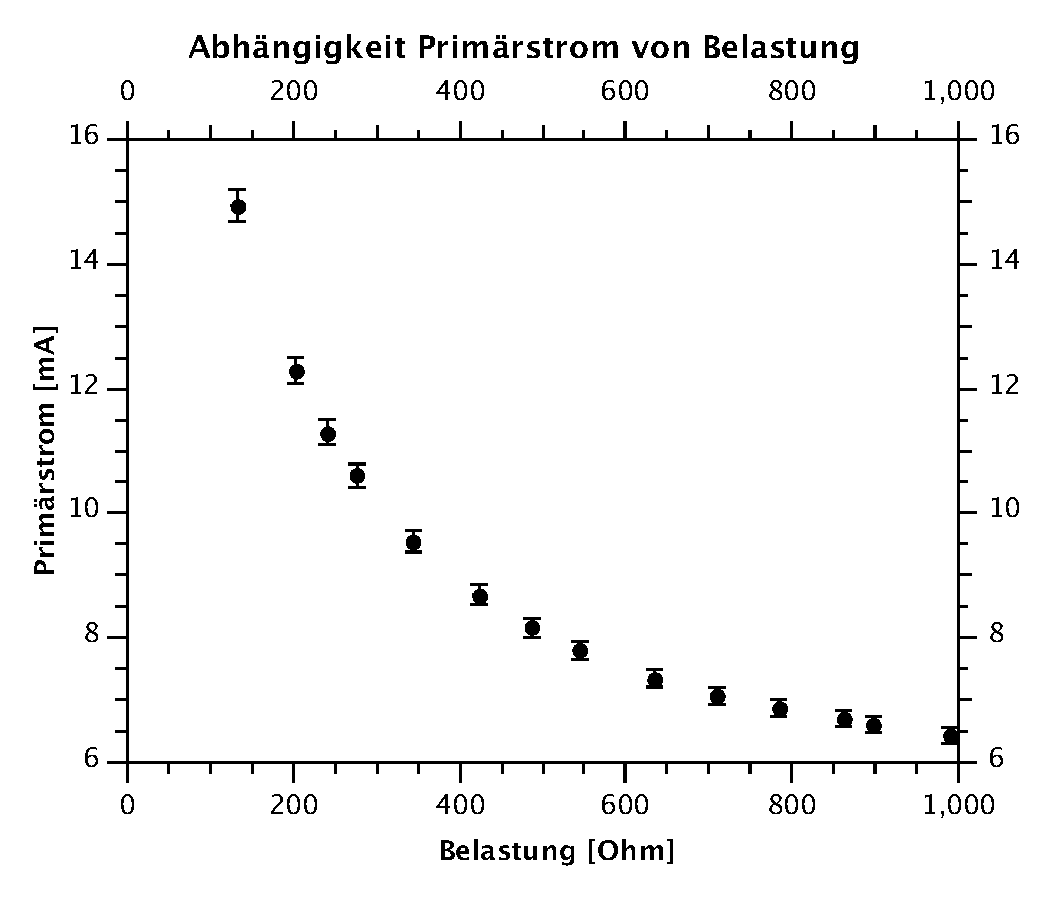
\includegraphics[scale=0.6]{Plot-Strom-Belastung.eps}
\end{figure}
\begin{figure}
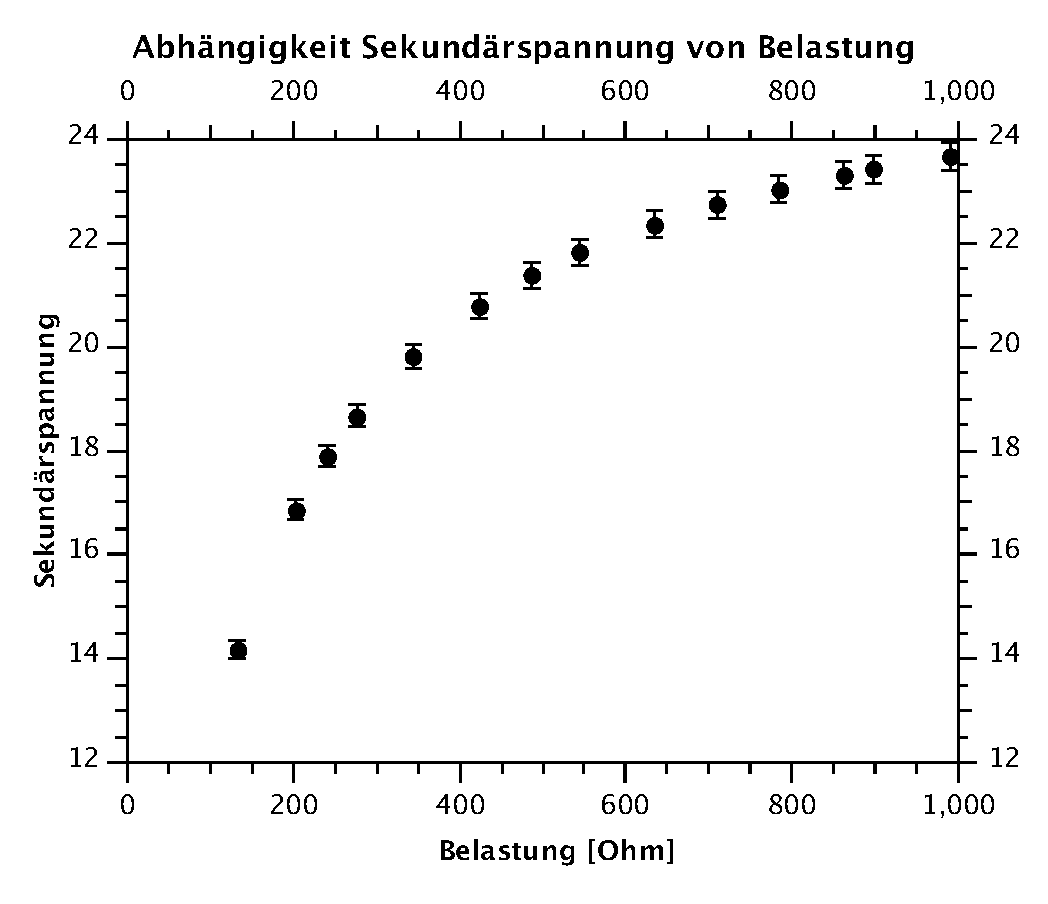
\includegraphics[scale=0.6]{Plot-Spannung-Belastung.eps}
\end{figure}

\subsection{Diskussion}
\textbf{Belastung:}\\
%Was können Sie über den Phasenwinkel eines unbelasteten Transformators sagen?
Der Phasenwinkel eines unbelasteten Transformators ist $\frac{\pi}{2}=90^\circ$.\\
\\
%Welche (Mess-)Größe existiert nur bei Belastung?
Der Strom in der Sekundärspule existiert nur bei Belastung, da ohne Belastungswiderstand der Stromkreis der Sekundärseite nicht geschlossen ist. \\
Diese Frage hatten wir schon vor dem Praktikumstag beantwortet, darum ist es umso ungeschickter, dass wir unseren Fauxpas bei der Strommessung nicht gesehen haben.
\\
%Für welchen Belastungswiderstand ist die Leistungsanpassung optimal?
\textbf{Primärimpedanz:}\\
%Wann ist die Primärimpedanz rein induktiv, wenn man vom Ohm'schen Widerstand der Primärspule absieht?
Die Primärimpedanz ist (abgesehen vom Ohm'schen Widerstand der Primärspule) rein induktiv, wenn der Transformator unbelastet ist. (Kein Lastwiderstand an der Sekundärseite).\\
\\
\textbf{Fehlerabschätzung:}\\
%Welche Fehlerquellen beeinflussen unsere Messungen?
Wie in der Durchführung bereits beschrieben haben wir tatsächlich einen Fehler im wörtlichen Sinne begangen und diesen wie dort beschrieben ausgemerzt. Wir erkennen im Nachhinein, dass unsere im Praktikum durchgeführte Strommessung von $I_2=0.03mA$ höchstwahrscheinlich ein Fehler im Aufbau der Schaltung war. Wir vermuten, dass das Messgerät eigentlich den Strom durch das Voltmeter gemessen hat, das ja einen großen Innenwiderstand besitzt und daher kaum mehr Strom ins Ampèremeter fließt.\\
\\
Außerdem unvermeidbare Fehlerquellen sind solche Fehlerquellen, die durch die verwendeten Teile unseres Versuchsaufbaus auftreten: Nicht-lineares Verhalten des Regelwiderstandes, Schwankungen der Netzspannung und Verluste am Transformator (da wir Ohm'sche Verluste, Entstehung von Wirbelströmen, Streufelder, Hysterese nicht miteinbeziehen).
%Wie gehen die Fehler der beiden Messgeräte in die Messung ein?




\end{document}
